\question[10] Un artista construye un pedestal de madera para exhibir una escultura como el que se muestra en la figura \ref{fig:prob_verb_superficie_01}.
Planea recubrir el pedestal con mosaicos.
\textbf{¿Cuánto mosaico se requerirá para recubrir el pedestal, incluyendo la base?}

\begin{minipage}{0.3\linewidth}
    \begin{figure}[H]
        \begin{center}
            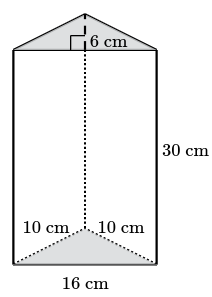
\includegraphics[width=0.8\textwidth]{../images/prob_verb_superficie_01}
        \end{center}
        \caption{}
        \label{fig:prob_verb_superficie_01}
    \end{figure}
\end{minipage}
\begin{minipage}{0.7\linewidth}
    % \begin{solutionbox}
    %     El volumen de un cilindro de radio $r$ y altura $h$ es:
    %     \begin{equation*}
    %         V = \pi r^2 h
    %     \end{equation*}
    %     De la figura \ref{fig:vol_area_03} se sabe que $r=2$ y $h=5$, entonces
    %     \begin{equation*}
    %         \begin{split}
    %             V & = \pi r^2 h\\
    %             & = \pi (4)^2 (10)\\
    %             & = \pi (16) (10)\\
    %             & = 160\pi
    %         \end{split}
    %     \end{equation*}
    % \end{solutionbox}
\end{minipage}